% ------------------------------------------------------------%
% 2015-2021 - Emerson Ribeiro de Mello <mello@ifsc.edu.br>
% ------------------------------------------------------------%
% Sets aspect ratio to 4:3, and frame size to 128 mm by 96 mm
\documentclass{beamer}
% Sets aspect ratio to 16:9, and frame size to 160 mm by 90 mm.
% \documentclass[aspectratio=169]{beamer}
% Sets aspect ratio to 16:10, and frame size to 160 mm by 100 mm.
% \documentclass[aspectratio=1610]{beamer}

% -------------------------------------------------%
%  Package options
% -------------------------------------------------%
% 
% textbgcolor   - frametitle background color. default: 0d4f4d
% textfgcolor   - frametitle foreground color. default: ffffff
% slidebgcolor  - slide background color. default: eef1ec
% slidefgcolor  - slide text foreground color. default: 000000
% authorfgcolor - author, institute and date color. default: 000000
% itemsep - space between items (itemize, enumerate). default: 7pt
\usepackage[textbgcolor=0d4f4d,textfgcolor=ffffff,itemsep=7pt]{beamerthemeifscyan}
% -------------------------------------------------%

% A good place to get some colors
% https://material.io/resources/color/#!/?view.left=0&view.right=0&primary.color=0d4f4d
% cyan: #0D4F4D, light: #417b79,  dark: #002625
% IFSC green: normal: #32A041, light: #69d26f, dark: #007013
% IFSC red: normal: #C8191E, light: #ff5747, dark: #8f0000 
% Other colors for textbgcolor
% purple 4527a0, blue 0d47a1, grey 546e7a, redwine 880e4f, brown 6d4c41, yelllow (bg=#fbc02d, fg=000000)

% Logo
\pgfdeclareimage[height=.4\paperheight]{ifsclogo}{img/ifsclogo.pdf}


% -------------------------------------------------%
%              Título 
% -------------------------------------------------%
\title{Tema IFSCyan para~\LaTeX~Beamer}
\subtitle{Nova organização para possibilitar personalizações}

\author{Prof. Emerson Ribeiro de Mello, Dr.}
\institute{%
\url{mello@ifsc.edu.br}%
}%
\date{16/07/2021}
% -------------------------------------------------%



% -------------------------------------------------%
%  Início do documento 
% -------------------------------------------------%
\begin{document}

\begin{frame}[plain]
    \titlepage
\end{frame}

\begin{frame}[plain, noframenumbering]{Licenciamento}
    \licenciamentoLivre
\end{frame}

\begin{frame}[plain, noframenumbering]{Sumário}
    \tableofcontents
\end{frame}



\section{Listas}


\begin{frame}{Lista de itens}
    \begin{enumerate}
        \item Primeiro item
        \begin{itemize}
            \item \Myhref{http://docente.ifsc.edu.br/mello}{Este texto é um \textit{link} para um site}
            \item Segundo item
        \end{itemize}
        \item Segundo item
        \item Terceiro item 
        \begin{itemize}
            \item Neste linha é apresentado um item que tem um texto grande que deverá ocupar mais de uma linha no slide. Assim, espera-se mostrar como será o alinhamento na margem esquerda
            \item Segundo item
        \end{itemize}
    \end{enumerate}
\end{frame}

\begin{frame}[wide]{Lista de itens com espaçamento 10pt}
    \begin{enumerate}
        \item Primeiro item
        \begin{itemize}
            \item \Myhref{http://docente.ifsc.edu.br/mello}{Este texto é um \textit{link} para um site}
            \item Segundo item
        \end{itemize}
        \item Segundo item
        \item Terceiro item 
        \begin{itemize}
            \item Neste linha é apresentado um item que tem um texto grande que deverá ocupar mais de uma linha no slide. Assim, espera-se mostrar como será o alinhamento na margem esquerda
            \item Segundo item
        \end{itemize}
    \end{enumerate}
\end{frame}

\subsection{Colunas}

\begin{frame}{Listas em colunas}
    \begin{columns}[t, onlytextwidth]
        \column{0.5\textwidth}
            \begin{itemize}
                \item Item 1
                \begin{itemize}
                    \item Subitem 1.1
                    \item Subitem 1.2
                \end{itemize}
                \item Item 2
                \item Item 3
            \end{itemize}
        
        \column{0.5\textwidth}
            \begin{enumerate}
                \item First
                \item Second
                \begin{enumerate}
                    \item Sub-first
                    \item Sub-second
                \end{enumerate}
                \item Third
            \end{enumerate}
    \end{columns}
\end{frame}


\section{Blocos}


\begin{frame}{Blocos}
    \begin{block}{Esse é um bloco}
        Isso é um teste
    \end{block}
    \begin{block}{}
    Bloco sem título	
    \end{block}
    \begin{alertblock}{Alerta}
        Esse é um alerta
    \end{alertblock}
    \begin{exampleblock}{Bloco para exemplo}
           Um bloco para usar com exemplos
        \end{exampleblock}
\end{frame}

\begin{frame}{Blocos personalizados}
\begin{atencao}
    Isso é uma mensagem de atenção
\end{atencao}
\begin{informacao}
    Isso é uma mensagem de informação
\end{informacao}
\begin{cuidado}
    Isso é uma mensagem de cuidado
\end{cuidado}

\end{frame}

\section{Figuras}

\begin{frame}{Figura 4x3}
    \begin{center}
        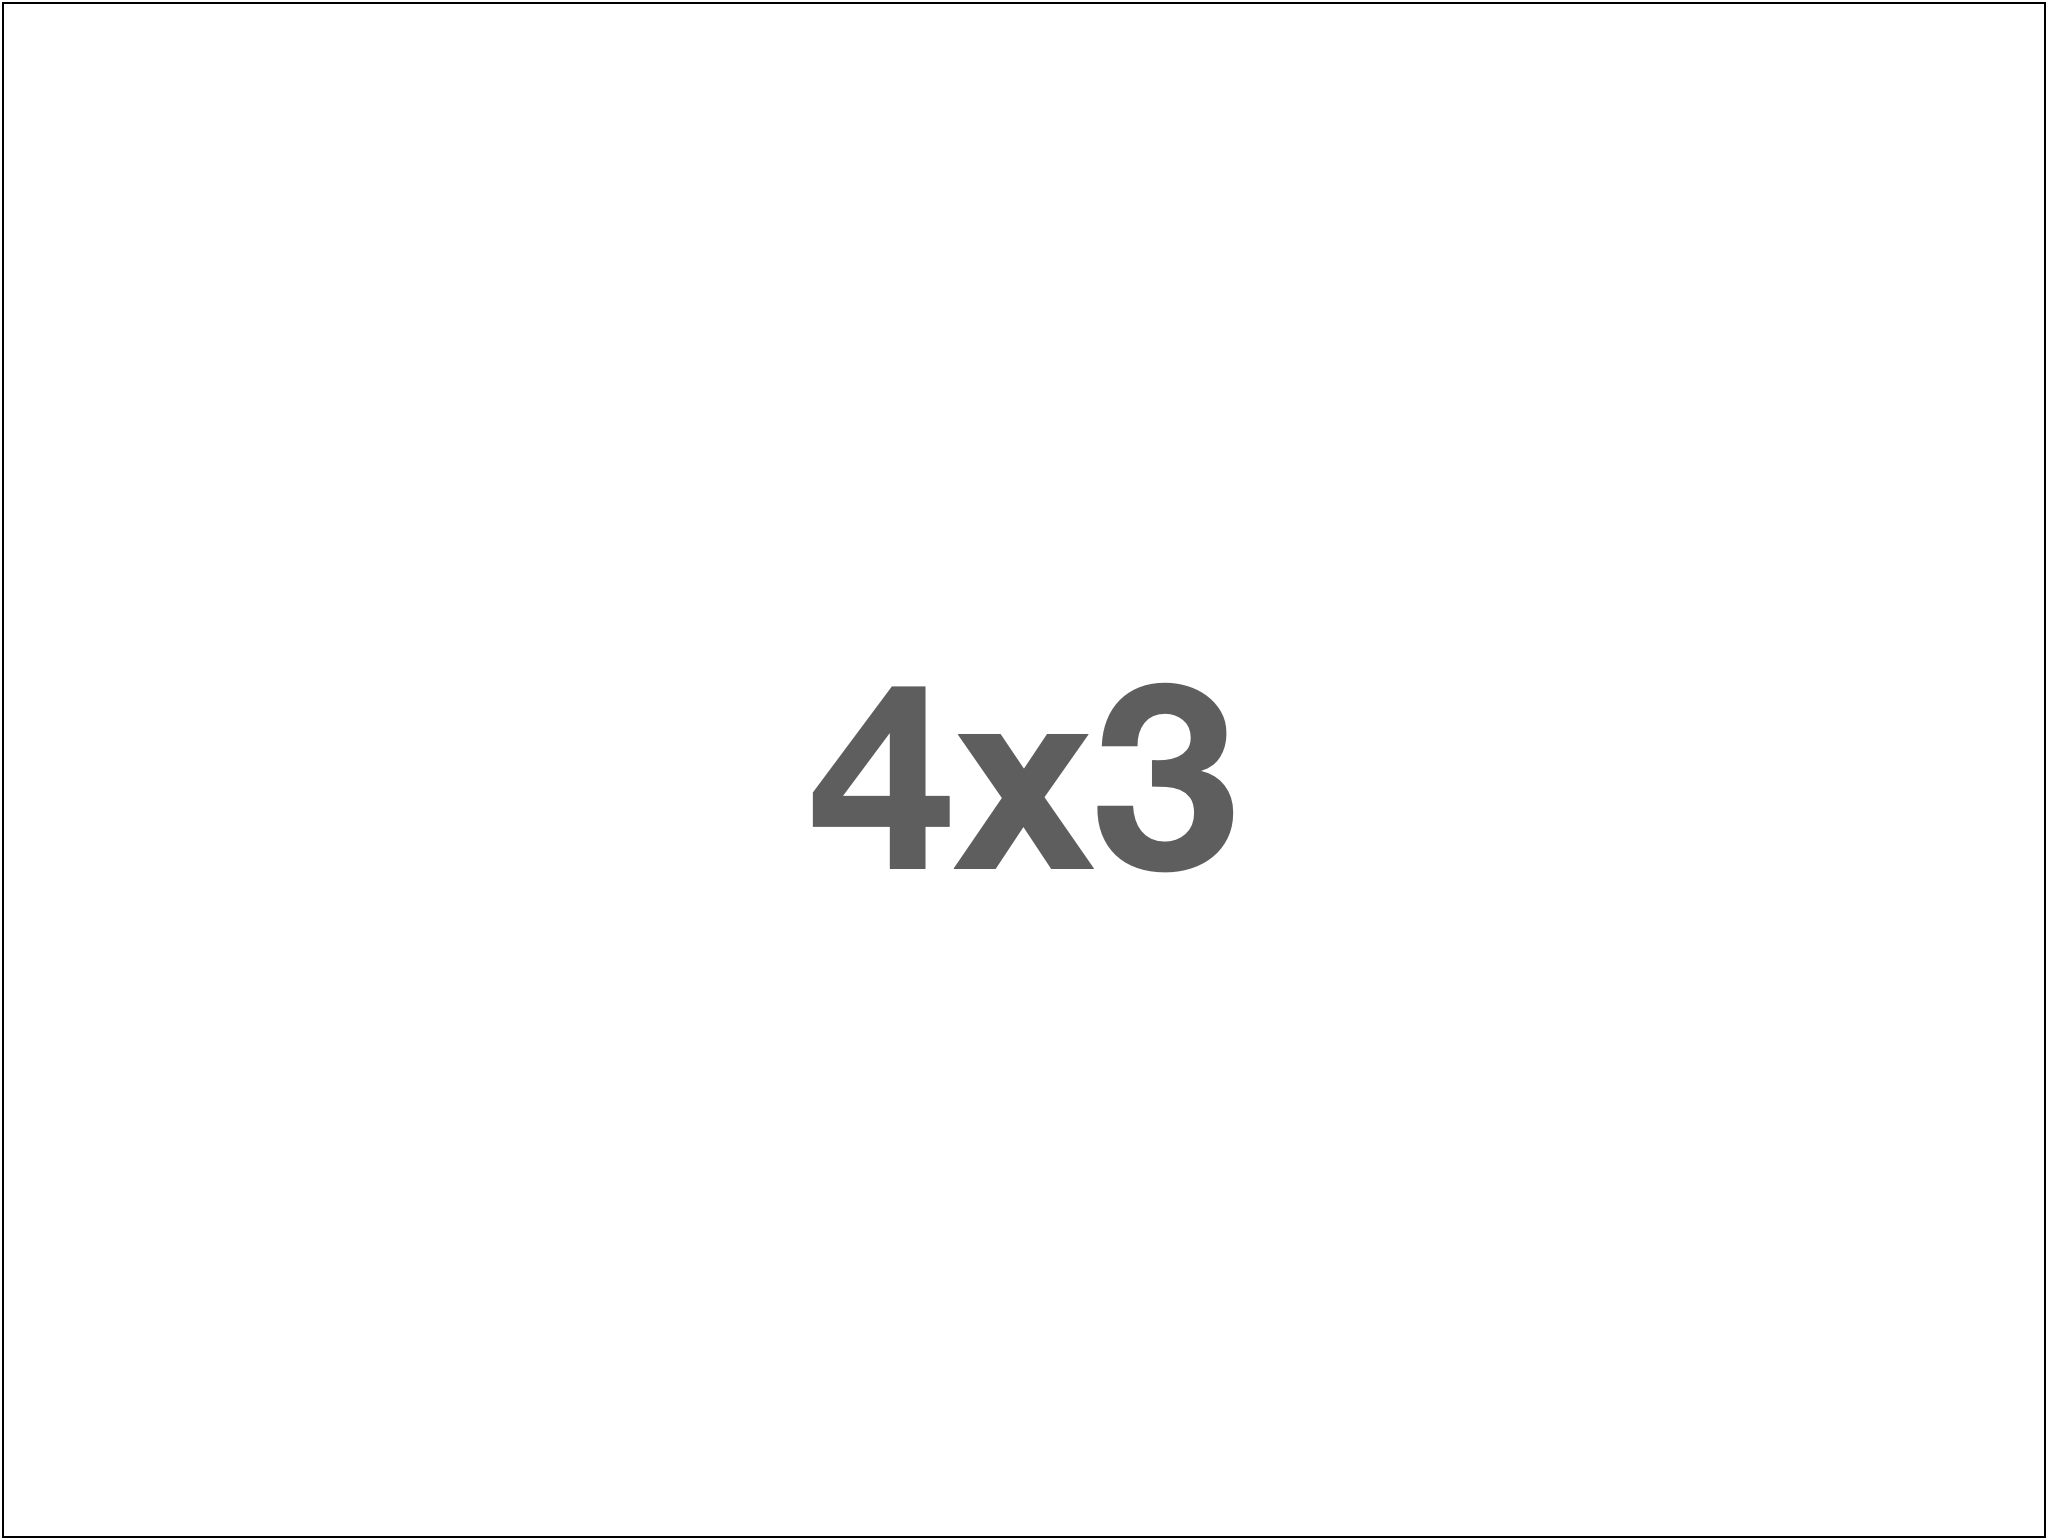
\includegraphics[width=.8\linewidth]{figs/4x3.png}
    \end{center}
\end{frame}
    

\begin{frame}{Figura 16x9}
\begin{center}
    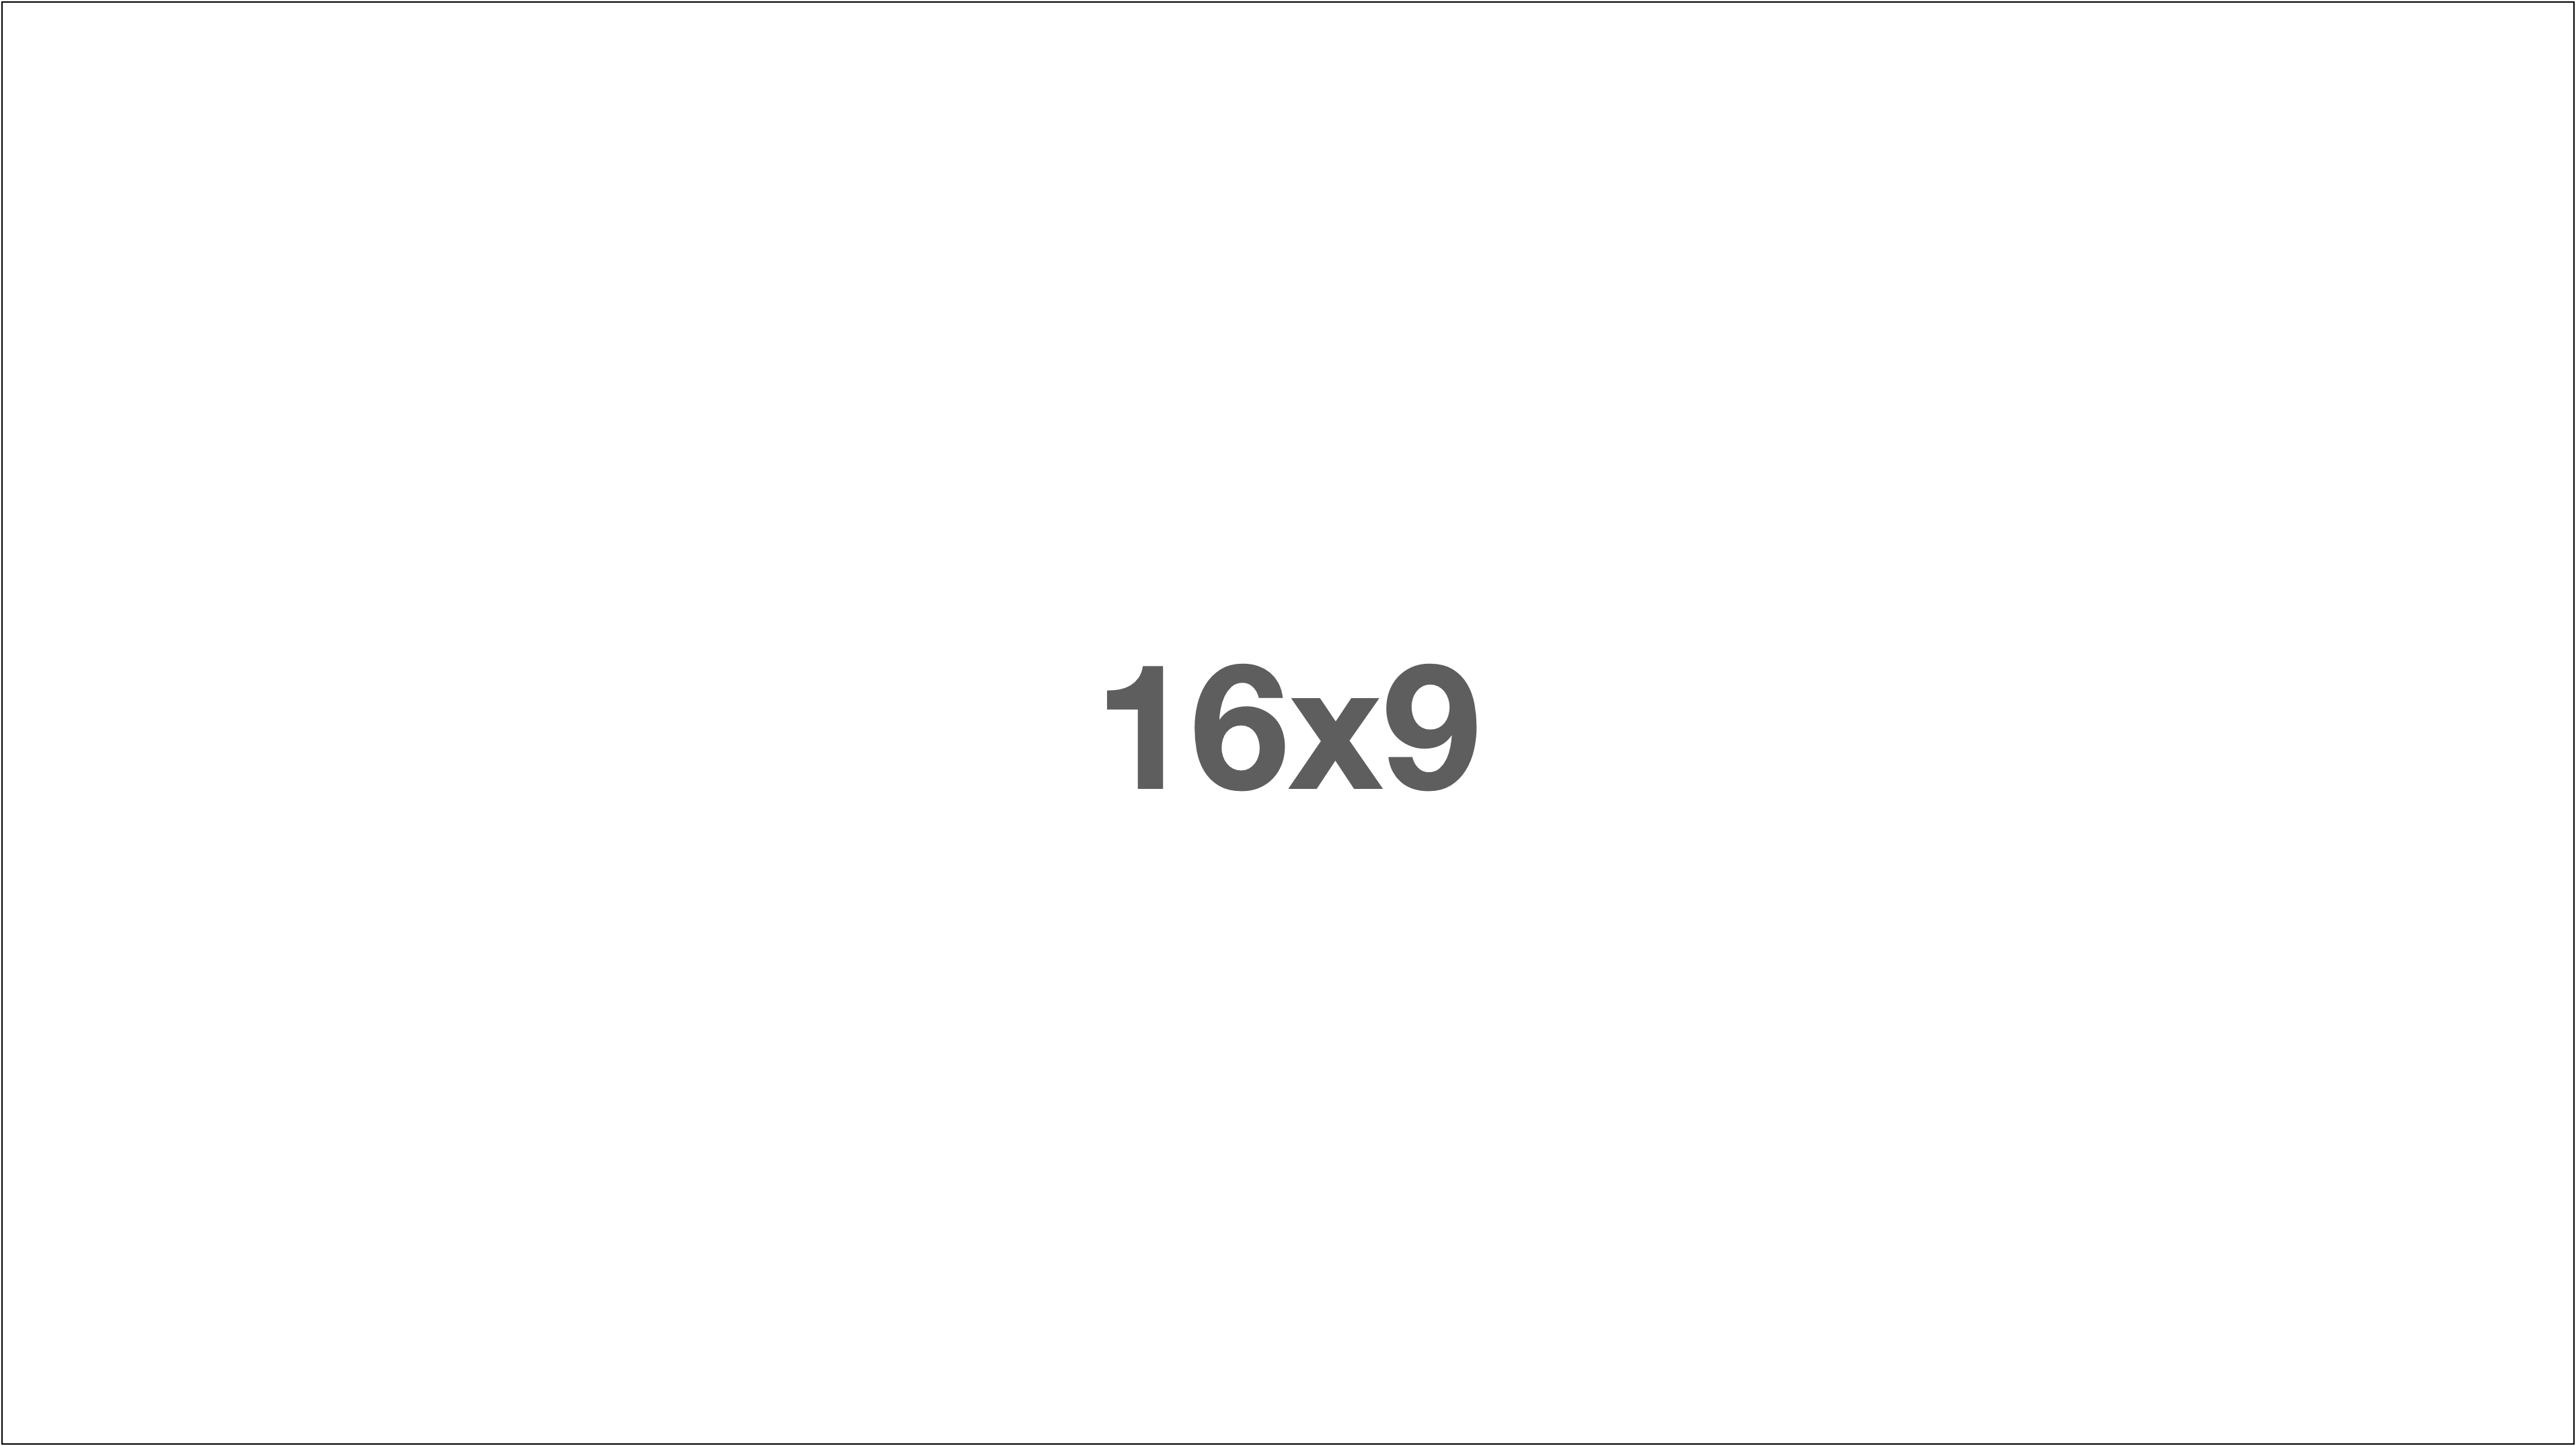
\includegraphics[width=\linewidth]{figs/16x9.png}
\end{center}
\end{frame}

\section{Tabelas}

\begin{frame}{Tabelas}
\begin{center}
    \begin{tabular}{l r r}\\\toprule
        Produto & Quantidade & Valor (R\$) \\\midrule
        Água    &      100   &   1,50 \\ 
        Banana  &       10   &   3,00 \\
        Maça    &        1   &   2,50 \\ \bottomrule
    \end{tabular}
\end{center}
\end{frame}






\begin{frame}[fragile]{Código em C e Java}

\begin{itemize}
		\item Comandos criados para as seguintes linguagens
		\begin{itemize}
			\item \texttt{ansic, java, shell, php, matlab, python, xml, sql}
			\item \texttt{ansicp, javap, shellp, phpp, matlabp, pythonp, xmlp, sqlp}
			\item Letra p no final indica que a fonte será \texttt{scriptsize}
		\end{itemize}
\end{itemize}

% -------------------------------------------------%
% incluindo o código de um arquivo externo
% -------------------------------------------------%
\includecode{ansic}{codigos/ola.c}	


% -------------------------------------------------%
% escrevendo o código diretamente dentro do frame
% -------------------------------------------------%
\javap
\begin{lstlisting}
public static voi main(String args[]){
	System.out.println("Ola mundo");
}
\end{lstlisting}		
\end{frame}
    

\begin{frame}{Referências}
    \nocite{*}
    \bibliography{demo_bibliography}
    \bibliographystyle{plain}
\end{frame}

\appendix

\section{Slides de backup}

\begin{frame}{Slide de backup}
    \usebeamercolor[fg]{normal text}
    Slides de backup são úteis para incluir materiais adicionais, necessários somente para ajudar a responder possíveis perguntas da plateia
    \vfill
    O pacote \texttt{appendixnumberbeamer} é usado para não numerar os slides de backup
\end{frame}


\end{document}